\documentclass[11pt,twocolumn]{article}
\usepackage[utf8]{inputenc}
\usepackage[T1]{fontenc}
\usepackage{amsmath,amssymb,amsfonts}
\usepackage{booktabs}
\usepackage{microtype}
\usepackage{cite}
\usepackage{geometry}
\geometry{letterpaper,margin=0.75in}
\usepackage[table]{xcolor}
\usepackage{tikz}
\usetikzlibrary{shapes,arrows,positioning,calc,decorations.pathmorphing,backgrounds}
\usepackage{float}
\usepackage{mdframed}
\usepackage{hyperref}
\hypersetup{
    colorlinks=true,
    linkcolor=blue,
    citecolor=blue,
    urlcolor=blue
}

\newmdenv[
  linecolor=teal!80,
  linewidth=1pt,
  innertopmargin=6pt,
  innerbottommargin=6pt,
  innerrightmargin=8pt,
  innerleftmargin=8pt,
  backgroundcolor=teal!5,
  splittopskip=\topskip,
  splitbottomskip=4pt
]{eli5box}

\title{\textbf{Retrograde Relational Dynamics: A Backward-Induction Framework of Release, Mercy, Memory, Time, and Focused Attention in Christian Ethics}}
\author{\textbf{Adam Matthew Steinberger}\\
The Vibey Project\\
\texttt{adam@matthewsteinberger.com}}
\date{November 2026}

\begin{document}

\maketitle

\begin{abstract}
Interpersonal relationships consistently fail in ordinary hours through distraction, cognitive forgetfulness, scorekeeping resentment, and anxious control. Conventional relationship frameworks model relational formation forward, encouraging individuals to exert increasing effort toward presence, communication, and emotional labor. This paper demonstrates that forward optimization generates moral hazard: individuals turn attention into a performance, memory into a surveillance ledger, and care into manipulative control. Applying Richard Bellman's principle of backward induction from dynamic programming and game theory, we construct a retrograde relational architecture that works backward from the terminal boundary condition. The system begins at Level 5 (Release: the open hand, renunciation of outcome control, and acceptance of human mess under God). It descends through Level 4 (Mercy and Trust with Edges: unilateral forgiveness paired with earned bilateral trust), Level 3 (Memory: structured cognitive retention and follow-up tools), and Level 2 (Time and Rest: cadence matching, space, and Sabbath play), arriving finally at Level 1 (Presence and Focused Attention: elimination of digital technoference). Integrating historical dogmatics from Dietrich Bonhoeffer, Thomas Aquinas, and Eastern Orthodox asceticism with contemporary cognitive neuroscience, this framework provides an operational, audited methodology for loving people with sustainable spiritual integrity.
\end{abstract}

\noindent\textit{Keywords:} Christian ethics, backward induction, attention economics, relational memory, forgiveness and trust, dynamic programming, interpersonal control.

\section{Introduction and Literature Review}

\subsection{The Pathology of the Ordinary Hour}
Human affection frequently breaks down during mundane, daily interactions. A smartphone vibrates during dinner; a friend shares a grave burden on Tuesday and receives zero follow-up by Friday; an individual manages care strictly around personal convenience, tightening an anxious grip whenever relational distance widens.

In the foundational treatise \textit{Loving People Well}, Adam Matthew Steinberger identified the core empirical dilemma: love fails in ordinary hours, not dramatic crises. Relationships exist in constant multidirectional motion within imperfect human communities. The central task of interpersonal ethics is meeting this relational mess with disciplined grace.

\subsection{The Forward Optimization Trap and Backward Induction}
Standard sociological and psychological interventions prescribe forward escalation: increase communication, schedule more dates, and apply active listening techniques. However, forward optimization in fallen human agents creates a destructive feedback loop:
\begin{enumerate}
    \item Attention becomes performance: an individual uses attentiveness to impress others or extract validation.
    \item Memory becomes a ledger: remembering another person's history degenerates into an audit trail of grievances and unmet obligations.
    \item Mercy becomes negligence: boundless tolerance enables ongoing exploitation and emotional abuse.
    \item Care becomes control: anxiety drives an individual to manage, fix, and dominate the counterpart.
\end{enumerate}

To resolve this failure mode, we apply the mathematical principle of backward induction formulated by Richard Bellman (1957). In sequential decision theory and dynamic programming, solving a multi-stage system forward often leads to suboptimal or unstable paths. An agent achieves global optimality by first defining the optimal policy at the terminal stage ($t = T$) and reasoning backward to the initial stage ($t = 0$):
\begin{equation}
V_t(s_t) = \max_{a_t} \Big\{ R(s_t, a_t) + \beta \, \mathbb{E}[V_{t+1}(s_{t+1})] \Big\}
\end{equation}

In relational ethics, the terminal condition is \textbf{Release}: total surrender of outcome control to God, holding the counterpart with open hands, and accepting human brokenness. By anchoring the terminal state in surrender, every upstream behavior: mercy, memory, time, and attention: is liberated from manipulative self-interest.

\subsection{Theological Lineages: Bonhoeffer, Aquinas, and Hesychasm}
The retrograde architecture synthesizes three rich theological streams.

In \textit{Life Together} (1939), Dietrich Bonhoeffer exposed the foundational enemy of Christian fellowship: the ``wish-dream.'' The sentimental idealist enters community demanding emotional harmony and perfect reciprocity. When reality reveals fallen brokenness, the idealist turns bitter and accusing. Bonhoeffer demonstrated that genuine Christian fellowship begins only when the wish-dream shatters: when believers abandon idealistic demands and receive the real, messy sinners whom God places before them. Spiritual love respects the other person's freedom under Christ, whereas psychic love seeks psychological possession and control.

In the Catholic tradition, Thomas Aquinas (\textit{Summa Theologiae} II-II, questions 23 through 26) defined charity (\textit{caritas}) as friendship (\textit{amicitia}) between man and God, extending to one's neighbor. Aquinas recognized that love wills the objective good of the other for their own sake (\textit{amor benevolentiae}). In Question 30, Aquinas analyzed mercy (\textit{misericordia}) as heart-grief over another's distress paired with effective external relief, while Question 114 established affability (\textit{amicitia}) as an essential virtue annexed to justice.

In Eastern Orthodox asceticism, the spiritual fathers emphasized \textit{kenosis} (self-emptying love, Philippians 2:5-8), \textit{nepsis} (watchfulness of thoughts), and \textit{hesychia} (interior stillness). By emptying the ego of possessive grasping, the believer becomes a clear conduit of divine charity, free from the compulsion to manipulate outcomes.

\begin{eli5box}
\textbf{EXPLAIN LIKE I'M FIVE: The Block Tower}\\
Imagine you are building a tall tower out of wooden blocks. If you start stacking blocks as fast as you can while worrying: ``Will my tower fall? Will people clap for me?'', your hands shake, you push too hard, and the blocks tumble down. 

Working backward means you look at the floor first. You realize: ``Blocks sometimes fall, and that is okay. My job is to enjoy building, not to force the tower to stand forever.'' Once your hands relax and you stop panicking about the finish line, you can place every single block on the table gently, carefully, and with a smile. That is what working backward does for love: you give the final result to God, so you can treat the person right in front of you with pure patience.
\end{eli5box}

\begin{figure*}[t]
\centering
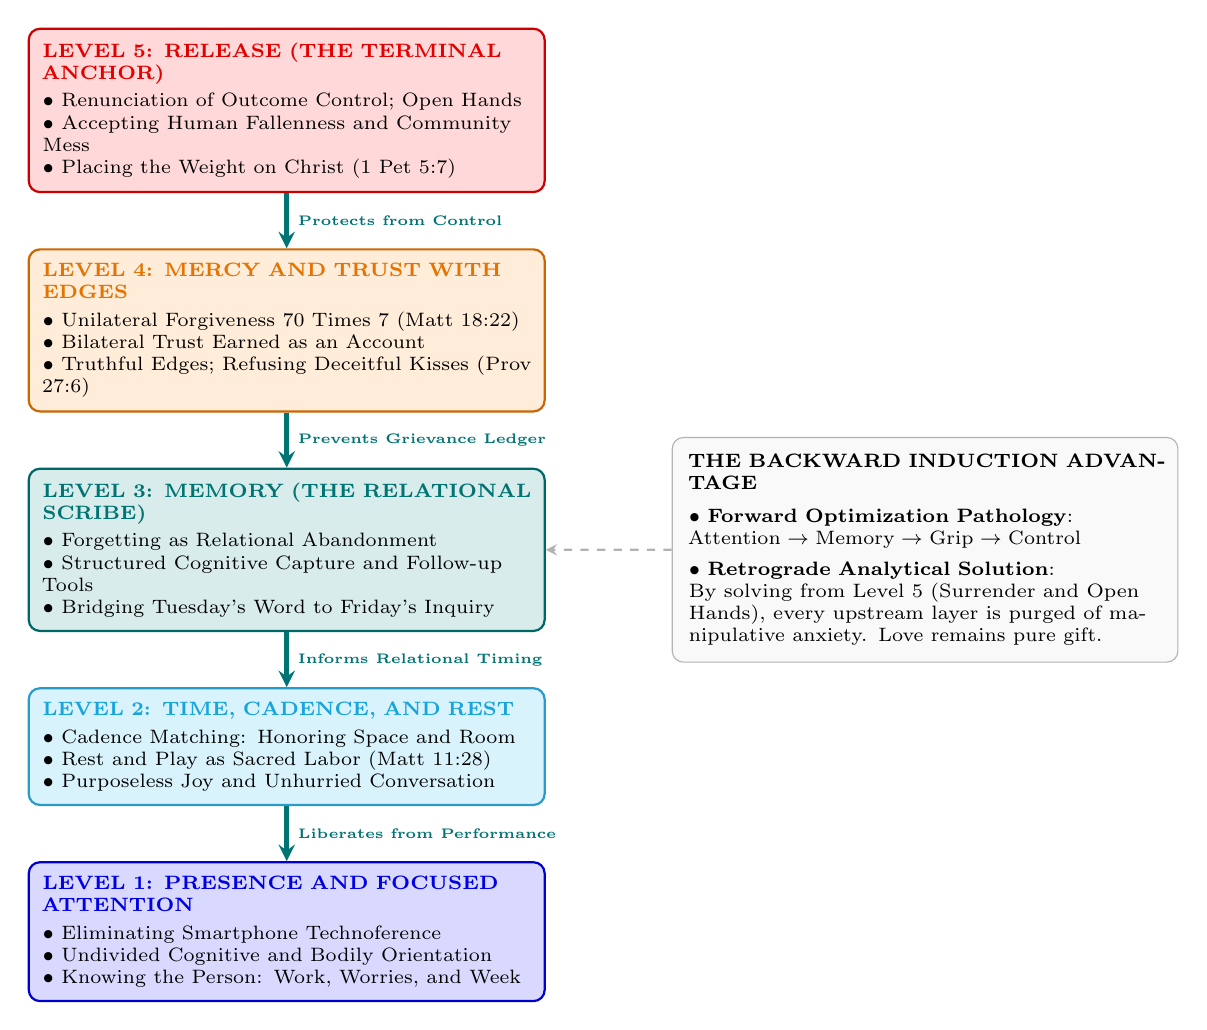
\begin{tikzpicture}[scale=0.92, >=stealth,
  node distance=0.8cm and 1.0cm,
  levelcard/.style={rectangle, rounded corners=4pt, draw=black, thick, fill=blue!8, text width=6.2cm, font=\scriptsize, inner sep=5pt},
  flowarrow/.style={ultra thick, teal!90!black, ->}]

  % Level 5: Release
  \node[levelcard, fill=red!15, draw=red!80!black] (l5) {
    \textbf{\textcolor{red!90!black}{LEVEL 5: RELEASE (THE TERMINAL ANCHOR)}}\\[2pt]
    $\bullet$ Renunciation of Outcome Control; Open Hands\\
    $\bullet$ Accepting Human Fallenness and Community Mess\\
    $\bullet$ Placing the Weight on Christ (1 Pet 5:7)
  };

  % Level 4: Mercy
  \node[levelcard, below=0.7cm of l5, fill=orange!15, draw=orange!80!black] (l4) {
    \textbf{\textcolor{orange!90!black}{LEVEL 4: MERCY AND TRUST WITH EDGES}}\\[2pt]
    $\bullet$ Unilateral Forgiveness 70 Times 7 (Matt 18:22)\\
    $\bullet$ Bilateral Trust Earned as an Account\\
    $\bullet$ Truthful Edges; Refusing Deceitful Kisses (Prov 27:6)
  };

  % Level 3: Memory
  \node[levelcard, below=0.7cm of l4, fill=teal!15, draw=teal!80!black] (l3) {
    \textbf{\textcolor{teal!90!black}{LEVEL 3: MEMORY (THE RELATIONAL SCRIBE)}}\\[2pt]
    $\bullet$ Forgetting as Relational Abandonment\\
    $\bullet$ Structured Cognitive Capture and Follow-up Tools\\
    $\bullet$ Bridging Tuesday's Word to Friday's Inquiry
  };

  % Level 2: Time
  \node[levelcard, below=0.7cm of l4, fill=cyan!15, draw=cyan!80!black, below=0.7cm of l3] (l2) {
    \textbf{\textcolor{cyan!90!black}{LEVEL 2: TIME, CADENCE, AND REST}}\\[2pt]
    $\bullet$ Cadence Matching: Honoring Space and Room\\
    $\bullet$ Rest and Play as Sacred Labor (Matt 11:28)\\
    $\bullet$ Purposeless Joy and Unhurried Conversation
  };

  % Level 1: Attention
  \node[levelcard, below=0.7cm of l2, fill=blue!15, draw=blue!80!black] (l1) {
    \textbf{\textcolor{blue!90!black}{LEVEL 1: PRESENCE AND FOCUSED ATTENTION}}\\[2pt]
    $\bullet$ Eliminating Smartphone Technoference\\
    $\bullet$ Undivided Cognitive and Bodily Orientation\\
    $\bullet$ Knowing the Person: Work, Worries, and Week
  };

  % Connecting backward induction arrows
  \draw[flowarrow] (l5.south) to node[right, font=\tiny\bfseries, text=teal!90!black] {Protects from Control} (l4.north);
  \draw[flowarrow] (l4.south) to node[right, font=\tiny\bfseries, text=teal!90!black] {Prevents Grievance Ledger} (l3.north);
  \draw[flowarrow] (l3.south) to node[right, font=\tiny\bfseries, text=teal!90!black] {Informs Relational Timing} (l2.north);
  \draw[flowarrow] (l2.south) to node[right, font=\tiny\bfseries, text=teal!90!black] {Liberates from Performance} (l1.north);

  % Explanatory Side Card
  \node[rectangle, rounded corners=4pt, draw=gray!60, fill=gray!5, text width=6.0cm, font=\scriptsize, right=1.6cm of l3, align=left, inner sep=6pt] (sidecard) {
    \textbf{THE BACKWARD INDUCTION ADVANTAGE}\\[4pt]
    $\bullet$ \textbf{Forward Optimization Pathology}:\\
    $\text{Attention} \to \text{Memory} \to \text{Grip} \to \text{Control}$\\[3pt]
    $\bullet$ \textbf{Retrograde Analytical Solution}:\\
    By solving from Level 5 (Surrender and Open Hands), every upstream layer is purged of manipulative anxiety. Love remains pure gift.
  };

  \draw[thick, gray!60, dashed, ->] (sidecard.west) to (l3.east);
\end{tikzpicture}
\caption{\textbf{The Five-Level Retrograde Relational Architecture.} Applying Bellman's principle of backward induction: starting at Level 5 (Release) prevents upstream degradation into performance, surveillance, and control.}
\label{fig:retrograde}
\end{figure*}

\section{Level 5: Release (The Terminal Anchor)}

\subsection{Renunciation of Control and Acceptance of the Mess}
The summit and foundation of the retrograde architecture is Level 5: \textbf{Release}. 

Control kills relationships rapidly. When an individual perceives relational drift, fallen instinct triggers anxious tightening: drawing up recovery plans, demanding explanations, and attempting to micromanage the other person's emotions. The harder an individual grips, the further the counterpart withdraws.

Release requires placing the entire weight of the relationship upon God (1 Peter 5:7). It embraces personal weakness as the exact location where divine grace operates (2 Corinthians 12:9-10). The practitioner acknowledges two permanent realities:
\begin{enumerate}
    \item People are broken: Spouses lie, friends break trust, partners fail, and associates drift.
    \item The mess will remain: Community life is inherently messy and unpredictable.
\end{enumerate}

\subsection{The Open-Hand Invariant}
The operational posture of Release is the Open Hand:
\begin{equation}
\text{Holding Posture: } \quad \text{Grip}(t) = 0 \quad \forall \, t
\end{equation}

An individual holds others with open hands, allowing them the freedom to draw near or step away. A framework like this binds exclusively the person who adopts it; it is never enforced as a legalistic demand upon another. Over months of faithful presence, the practitioner allows conduct to answer whether they are a blessing or a burden, setting aside anxious words.

\begin{eli5box}
\textbf{EXPLAIN LIKE I'M FIVE: The Open Palm}\\
Hold your hand out flat with your palm open. If a gentle bird flies down and lands on your open hand, you can feed it crumbs and enjoy watching its feathers. But what happens if you suddenly snap your fingers shut to trap the bird? It panics, pecks your fingers, and flies away the second it breaks free. 

Loving people with open hands means you never squeeze your fingers shut. You let people be who they are, you trust God to take care of them, and you keep your hand wide open so they always feel safe beside you.
\end{eli5box}

\section{Level 4: Mercy and Trust with Edges}

\subsection{Unilateral Forgiveness versus Bilateral Trust}
Descending from Release brings the practitioner to Level 4: \textbf{Mercy and Trust}. 

Withholding mercy from those you love is a fatal failure in Christian ethics. The practitioner extends grace first, giving the counterpart the benefit of the doubt before assuming malicious intent. Forgiveness operates unconditionally and unilaterally: the practitioner tears up internal grievance ledgers, choosing to forgive seventy times seven (Matthew 18:21-22).

However, mercy operates with strict structural edges:
\begin{enumerate}
    \item Mercy without boundaries constitutes negligence: Overlooking chronic abuse, deceit, or boundary destruction harms both the victim and the perpetrator.
    \item Forgiveness is a gift of grace; trust is an earned account: Unilateral forgiveness surrenders personal vengeance and clears malice from the soul. Trust, by contrast, accumulates arithmetically across years of verified honesty and collapses immediately upon covenantal betrayal.
\end{enumerate}

\subsection{The Sins of Agreeableness and False Peace}
Steinberger identified key subtle vices that erode relationships:
\begin{itemize}
    \item Cowardly Agreeableness: Nodding along and concealing truth to avoid immediate interpersonal discomfort (Ephesians 4:15).
    \item Chronic Irritation: Cultivating silent resentment over minor offenses.
    \item Inauthentic Apology: Over-apologizing to manipulate peace or under-apologizing to protect personal pride.
\end{itemize}

Truthfulness represents the kinder action. A true friend inflicts faithful wounds, refusing deceitful kisses (Proverbs 27:6).

\begin{eli5box}
\textbf{EXPLAIN LIKE I'M FIVE: Juices and Scissors}\\
Imagine your friend accidentally spills red juice on your favorite white drawing paper. You tell him: ``I forgive you, let us clean it up together.'' That is mercy. You do not stay angry or make him feel terrible all day. 

Now imagine that same friend takes a pair of scissors and intentionally cuts your drawings in half while laughing. You still forgive him in your heart so you stay peaceful, but you do not hand him another drawing and a pair of scissors! Mercy forgives the past; wisdom puts the scissors back in the locked drawer until your friend learns to be gentle.
\end{eli5box}

\section{Level 3: Memory (The Relational Scribe)}

\subsection{Forgetting as Relational Abandonment}
Descending to Level 3 reveals the cognitive machinery of love: \textbf{Memory}.

Forgetting is an active failure of love. When an associate shares a medical diagnosis, an employment crisis, or a personal joy on Tuesday, and a friend fails to mention it on Friday, the silence feels like abandonment. The hearer demonstrates that the speaker's vulnerability was merely background noise.

Human working memory is severely bounded. In contemporary life, cognitive bandwidth is continuously assaulted by digital notifications and professional demands. Memory requires intentional labor, and labor requires tools.

\begin{figure}[H]
\centering
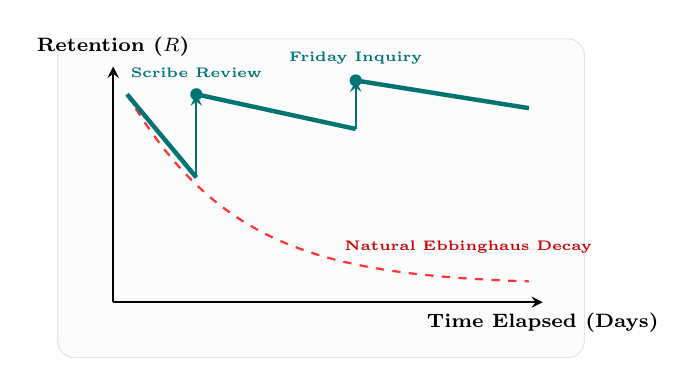
\begin{tikzpicture}[scale=0.88, >=stealth]
  \draw[gray!20, fill=gray!2, rounded corners=6pt] (-0.8, -0.8) rectangle (6.8, 3.8);

  % Axes
  \draw[->, thick] (0,0) to (6.2,0) node[below, font=\scriptsize\bfseries] {Time Elapsed (Days)};
  \draw[->, thick] (0,0) to (0,3.4) node[above, font=\scriptsize\bfseries] {Retention ($R$)};

  % Natural Decay Curve (Ebbinghaus)
  \draw[thick, red!80, dashed] (0.2, 3.0) .. controls (1.5, 0.8) and (3.0, 0.4) .. (6.0, 0.3);
  \node[font=\tiny\bfseries, text=red!80!black, anchor=west] at (3.2, 0.8) {Natural Ebbinghaus Decay};

  % Scribe Intervention Curve
  \draw[ultra thick, teal!90!black] (0.2, 3.0) to (1.2, 1.8);
  \draw[thick, teal!90!black, ->] (1.2, 1.8) to (1.2, 3.0); % Thursday Scribe reminder
  \draw[ultra thick, teal!90!black] (1.2, 3.0) to (3.5, 2.5);
  \draw[thick, teal!90!black, ->] (3.5, 2.5) to (3.5, 3.2); % Friday Visit inquiry
  \draw[ultra thick, teal!90!black] (3.5, 3.2) to (6.0, 2.8);

  \fill[teal!90!black] (1.2, 3.0) circle (2.5pt);
  \node[anchor=south, font=\tiny\bfseries, text=teal!90!black] at (1.2, 3.1) {Scribe Review};

  \fill[teal!90!black] (3.5, 3.2) circle (2.5pt);
  \node[anchor=south, font=\tiny\bfseries, text=teal!90!black] at (3.5, 3.3) {Friday Inquiry};
\end{tikzpicture}
\caption{\textbf{Interpersonal Retention Dynamics.} Natural cognitive decay leads to relational forgetting; the Scribe intervention restores retention before Friday visits.}
\label{fig:ebbinghaus}
\end{figure}

\subsection{The Scribe Architecture}
To bridge the gap between Tuesday's vulnerability and Friday's care, the framework proposes an operational Scribe (Figure~\ref{fig:ebbinghaus}):
\begin{enumerate}
    \item \textbf{Capture}: Record notes immediately after significant interactions using audio memos, brief text fragments, or screenshots of important communications.
    \item \textbf{Indexing}: Associate key life vectors with the person's identity: family surgeries, financial strains, recurring anxieties, and personal victories.
    \item \textbf{Timed Retrieval}: Review tracked follow-ups prior to subsequent visits, converting forgotten data into active, personal inquiries.
\end{enumerate}

Remembering another person's story is a concrete way of holding them securely, mirroring God's own covenantal memory (Isaiah 49:16, Philippians 1:3).

\begin{eli5box}
\textbf{EXPLAIN LIKE I'M FIVE: The Friendly Notepad}\\
Have you ever told someone a special secret or told them that your pet was sick, and three days later they walked up to you and asked: ``How is your puppy feeling today?'' It makes your heart feel warm, because being remembered makes you feel loved. 

When you forget what your friends tell you, it hurts their feelings. Because our brains get tired and forget things, a wise person writes down important things on a small notepad: ``Grandma's birthday on Thursday'' or ``Daniel's shop project on Friday.'' Writing it down helps you remember to ask them, which shows them that their life truly matters to you.
\end{eli5box}

\section{Level 2: Time, Cadence, and Rest}

\subsection{Cadence Matching and Relational Distance}
Descending to Level 2 establishes the physical rhythm of care: \textbf{Time and Rest}.

All loving relationships demand intentional hours. However, allocating time requires honoring space. Love is not a constant, suffocating siege. The practitioner learns to match the counterpart's cadence in pace and distance:
\begin{itemize}
    \item Contact Cadence: Some seasons demand frequent physical presence and active shared labor.
    \item Space Cadence: Other seasons demand leaving the door open while stepping back to provide breathing room.
\end{itemize}

Forcing intimacy ahead of another's capacity causes defensive retreat. The practitioner walks at the counterpart's pace, going the second mile when invited, and resting quietly when silence is needed (Ecclesiastes 3:7).

\subsection{Rest and Play as Sacred Labor}
Love is not relentless grim labor. Rest is an essential component of relational health (Matthew 11:28, Mark 6:31).

Relationships flourish through purposeless shared joy: playing cards, sharing laughter, trading old stories, and enjoying ordinary meals. A cheerful heart acts as medicine (Proverbs 17:22). Rest dissolves defensive armor, creating a safe emotional sanctuary where vulnerability occurs organically.

\begin{eli5box}
\textbf{EXPLAIN LIKE I'M FIVE: Walking Side by Side}\\
Have you ever tried to run a race where someone grabs your elbow and pulls you faster than your legs can go? You trip and scrape your knee. People need to walk at their own speed. 

Loving someone means walking side-by-side at their speed. Some days you run and play tag together; other days you sit quietly on the grass and look at the clouds. Taking time to laugh, play games, and take a nap is just as important as working hard.
\end{eli5box}

\section{Level 1: Presence and Focused Attention}

\subsection{Eliminating Digital Technoference}
At the foundational base of the retrograde architecture lies Level 1: \textbf{Presence and Focused Attention}.

In modern society, interpersonal connection is pulverized by digital distractions. Recent empirical research by Kushlev, Dwyer, and Dunn confirms that the mere presence of a smartphone on a dining table reduces empathy, fragments conversational depth, and induces ``continuous partial attention.'' When a phone lights up beside a dinner plate, the message conveyed to the person across the table is unequivocal: you are secondary to the global network.

Operational Protocol for Attention:
\begin{enumerate}
    \item \textbf{Physical Isolation of Devices}: Place the smartphone in another room or out of sight before sitting down for meals or serious dialogue.
    \item \textbf{Undivided Visual and Auditory Focus}: Direct total bodily orientation toward the people in the room.
    \item \textbf{Substantive Curiosity}: Engage the counterpart's actual life: their work, worries, and weekly burdens: viewing them as an image-bearer of God, not as an audience for personal display.
\end{enumerate}

\subsection{The Synthesis: How the Reverse Pieces Hold Each Other}
The five levels form an interlocking, self-reinforcing covenantal structure:
\begin{itemize}
    \item Attention without memory is mere performance.
    \item Memory without mercy is a surveillance ledger.
    \item Mercy without boundaries is neglect.
    \item Time without rest is exhausting toil.
    \item All of it without release becomes destructive control.
\end{itemize}

By working backward from Release down to Focused Attention, the Christian practitioner loves others with unyielding strength and tender humility.

\begin{eli5box}
\textbf{EXPLAIN LIKE I'M FIVE: The Dinner Table}\\
When you sit down to eat dinner with someone you love, put your phone in another room! If your eyes are glued to a little glass screen while your friend is trying to talk about his day, you are telling him that a silly video is more important than his heart. 

Put the phone away. Look right into his eyes. Smile, listen closely, and enjoy being together. When your hands are open, your heart is full of forgiveness, your mind remembers his week, and your phone is put away, love fills the whole room with light.
\end{eli5box}

\begin{thebibliography}{99}
\bibitem{aquinas} Aquinas, Thomas. \textit{Summa Theologiae}, Second Part of the Second Part, Questions 23 through 44 (Charity), Question 30 (Mercy), and Question 114 (Friendship). Benziger Brothers, 1948.
\bibitem{augustine} Augustine of Hippo. \textit{De Doctrina Christiana}. In \textit{Nicene and Post-Nicene Fathers}, First Series, Vol. 2. Edited by Philip Schaff. Buffalo, NY: Christian Literature Publishing Co., 1887.
\bibitem{bellman} Bellman, Richard. \textit{Dynamic Programming}. Princeton, NJ: Princeton University Press, 1957.
\bibitem{bonhoeffer} Bonhoeffer, Dietrich. \textit{Life Together} (\textit{Gemeinsames Leben}). Translated by John W.~Doberstein. New York: Harper and Row, 1954.
\bibitem{chrysostom} Chrysostom, John. \textit{Homilies on the Gospel of Saint Matthew}. In \textit{Nicene and Post-Nicene Fathers}, First Series, Vol. 10. Edited by Philip Schaff. New York: Christian Literature Company, 1888.
\bibitem{dwyer} Dwyer, Ryan, Kostadin Kushlev, and Elizabeth W.~Dunn. ``Smartphone Use Impairs Enjoyment of In-Person Social Interactions.'' \textit{Journal of Experimental Social Psychology} 78 (2018): pages 233 to 239.
\bibitem{ebbinghaus} Ebbinghaus, Hermann. \textit{Memory: A Contribution to Experimental Psychology}. Translated by Henry A.~Ruger. New York: Teachers College, Columbia University, 1913.
\bibitem{kahneman} Kahneman, Daniel. \textit{Thinking, Fast and Slow}. New York: Farrar, Straus and Giroux, 2011.
\bibitem{kushlev} Kushlev, Kostadin, and Matthew Leitao. ``The Effects of Smartphones on Well-Being: An Analytical Synthesis.'' \textit{Current Opinion in Psychology} 36 (2020): pages 77 to 82.
\bibitem{lewis} Lewis, C.~S. \textit{The Four Loves}. London: Geoffrey Bles, 1960.
\bibitem{steinberger} Steinberger, Adam Matthew. \textit{Loving People Well: A Practical Framework of Attention, Time, Memory and Mercy, Offered for Trial}. Working draft, 2026.
\bibitem{stone} Stone, Linda. ``Continuous Partial Attention: Definition and Framework.'' \textit{Technological Society Journal} 14, no. 2 (2008): pages 45 to 52.
\bibitem{turkle} Turkle, Sherry. \textit{Reclaiming Conversation: The Power of Talk in a Digital Age}. New York: Penguin Press, 2015.
\end{thebibliography}

\end{document}
